本システムは大きく分けて3つの機能によって成り立っている.
それは,グラフデータ管理機能,グラフデータ入力補助機能,グラフデータ可視化機能の3つの機能である.
それぞれの機能について\ref{subsec:kanri}節,\ref{subsec:hojo}節,\ref{subsec:kasi}節で説明する.

\subsection{グラフデータ管理機能}\label{subsec:kanri}
グラフデータ管理機能は,学習者と指導者のグラフデータを管理する機能で,クライアントのフォームから入力されたコンセプトマップの親子に関するデータをAPIを用いてグラフデータへと変換しグラフデータベースへとデータを登録する.
また,クライアントからグラフデータを要求された場合,グラフデータをAPIを用いてJSON形式で返答する.

グラフデータ管理機能が使用するAPIは以下のとおりである.

\begin{itemize}
    \item /create/json \\
    - 与えられたJSON形式のデータをグラフデータベースで利用できるJSON形式のデータに変換し,データを登録しその結果をJSON形式で返答する.

    \item /get/all\_graphs \\
    - グラフデータベースに登録されているすべてのグラフデータをJOSN形式で返答する.

    \item /create/score \\
    - 指定されたユーザと教科の点数登録を行う.

    \item /get/score \\
    - 指定された教科に紐づくすべての点数を返答する.

    \item /get/score/\<username\> \\
    - 指定されたユーザに関する教科の得点を返答する.

    \item /get/subject/\<subject\> \\
    - 指定されたユーザが受験した科目と点数を返答する.

    \item /delete/\<string:node\_name\> \\
    - 指定されたノードを削除する.

    \item /delete/all \\
    - すべてのノードを削除する.
    
\end{itemize}

これらのAPIを利用することにより本システムはグラフデータベースとコンセプトマップを紐づけて利用している.
\newpage

\subsection{グラフデータ入力補助機能}\label{subsec:hojo}

グラフデータ入力補助機能のGUIを図\ref{fig:hojo}に示す.

\begin{figure}[htbp]
\begin{center}
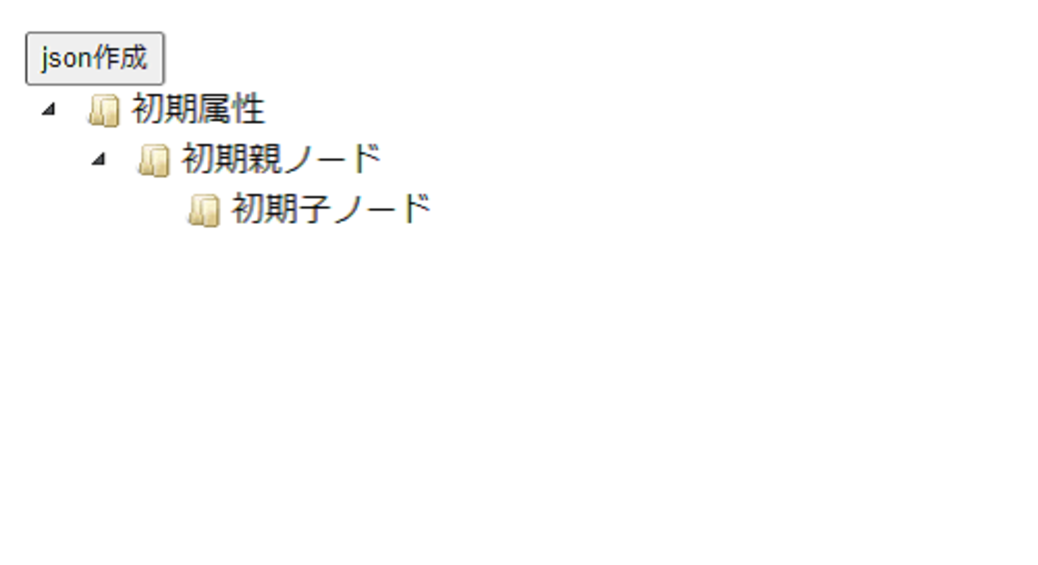
\includegraphics[width=10cm]{img/hojo.eps}
\end{center}
\caption{グラフデータ入力補助機能初期状態}
\label{fig:hojo}
\end{figure}

図\ref{fig:hojo}は初期状態で,図のような木構造な入力フォームを提示する.
初期属性とは第\ref{chap:conceptmap}章の図\ref{fig:example_concept}で示した植物に該当する.
初期親ノードは被子植物,初期子ノードはサクラに該当する.

各々の階層は図\ref{fig:hojo_change_name}のようにして各ノードを右クリックすることによりメニューが表示される.

\begin{figure}[htbp]
\begin{center}
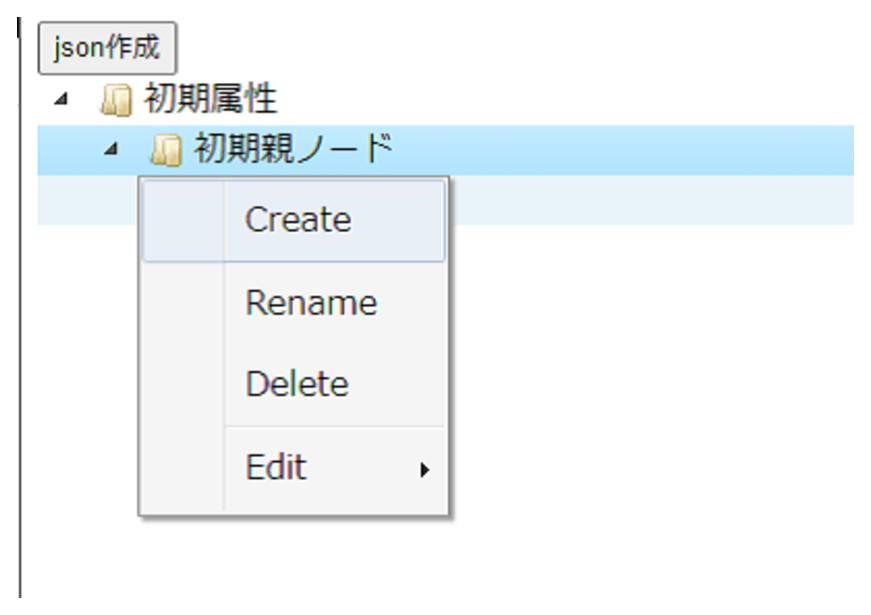
\includegraphics[width=10cm]{img/hojo_change_name.eps}
\end{center}
\caption{グラフデータ入力補助機能編集状態}
\label{fig:hojo_change_name}
\end{figure}

\subsection{グラフデータ可視化機能}\label{subsec:kasi}
